\chapter{Literature Review}
\label{chapter-literature-review}
\begin{ChapAbstract}
This chapter presents an overview of the literature in the virtual try-on and fashion recommendation fields. In the domain of virtual try-on, we introduce recent image virtual try-on approaches. Besides, some commercial products and their technology are discussed to provide a comprehensive view of this field. Moving on to fashion recommendation, we introduce related works centering on visual-based fashion recommendations. Finally, we discuss techniques for similarity search, including exhaustive and approximate methods applied to our recommendation approaches.
\end{ChapAbstract}
 %%%%%%%%%%%%%%%%%%%%%%%%%%%%%%%%%%%%%%%%%%%%%%%%%%%%%%%%%%%%%%%%
\section{Virtual Try-on}
This section presents the virtual try-on approaches, divided into two main parts. In the first one, we discuss the research on image-based virtual try-on, which aim to warp the garment to fit the target person's pose. After that, we introduce some commercial products that are being applied in practice and their limitations.

\subsection{Image-based Virtual Try-on}
Image-based virtual try-on techniques can be classified into two categories: parser-based and parser-free approaches, in the sense that they use a body-parser map in the inference process or not. Both of them typically involves three steps: extracting the intrinsic input features, warping the input garment to fit the clothing area of the person image, and performing the replacement using a generative model.

% \subsection{Parser-based Approach}
\paragraph{Parser-based Methods.} As for parser-based virtual try-on methods, they require human representation, including the human segmentation map, human pose, etc., to deform and fit the garment to the corresponding region on the input image. Previous methods~\cite{Han-CVPR2018-Viton, Wang-ECCV2018-Toward, Han-ICCV2019-Clothflow, Yang-CVPR2020-Towards, Fele-WACV2022-CVTON, Bai-ECCV2022-Single} utilized pretrained models such as human parsing~\cite{Gong-CVPR2017-Look, Li-TPAMI2020-Self}, pose estimation~\cite{Cao-CVPR2017-Realtime}, densepose~\cite{Guler-CVPR2018-DensePose} to extract information (i.e. human segmentation map) from the person input used for both training and inference.

The initial approach that laid the foundation for this method was VITON~\cite{Han-CVPR2018-Viton}, which proposed a coarse-to-fine framework. Firstly, a multi-task encoder-decoder generator is employed to generate a coarse sample and a clothing mask. Subsequently, the garment is warped using a thin plate spline (TPS) transformation with shape context matching. Finally, the coarse results are refined using a refinement network that leverages realistic details from a deformed item. Then it was realized that using image descriptors for warping had shown lower accuracy than deep learning networks. CP-VTON~\cite{Wang-ECCV2018-Toward}, building upon VITON~\cite{Han-CVPR2018-Viton}, adopted a similar architecture but utilized an end-to-end neural network to learn the transformation parameters of the TPS transformation. This improvement significantly enhanced the accuracy of the virtual try-on outcomes. 

\begin{figure}[h!]
    \centering
    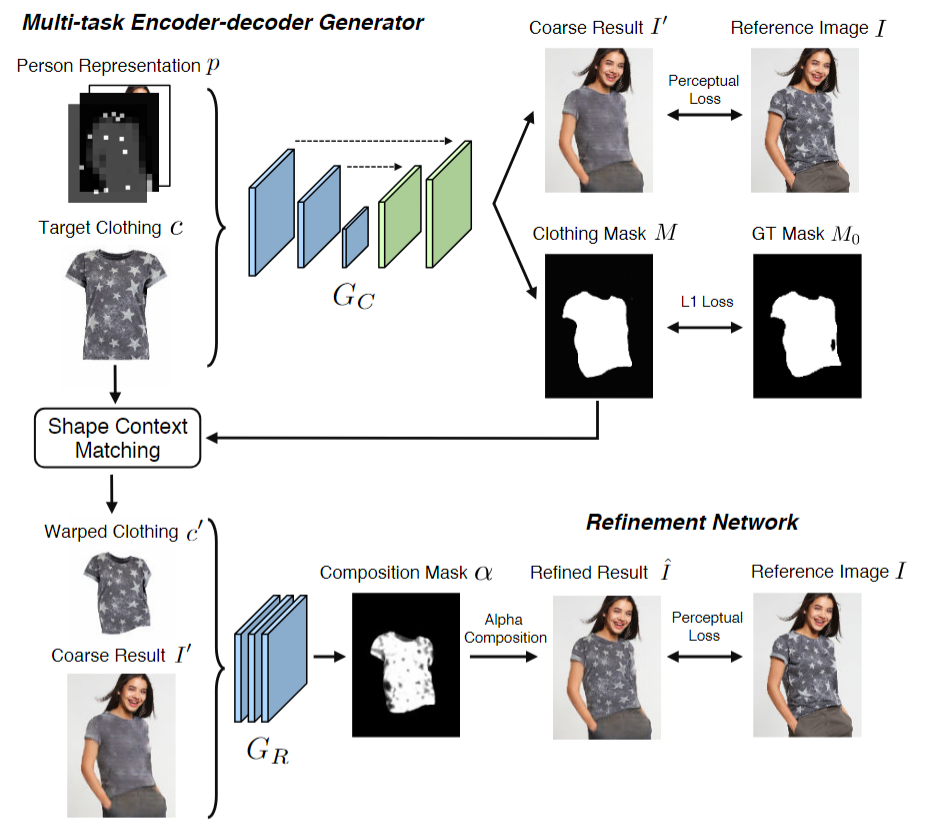
\includegraphics[width=0.7\linewidth]{content/resources/images/literature-review/viton.png}
    \caption{Overview architecture of VITON~\cite{Han-CVPR2018-Viton}.}
    \label{vton-viton}
\end{figure}

\begin{figure}[h!]
    \centering
    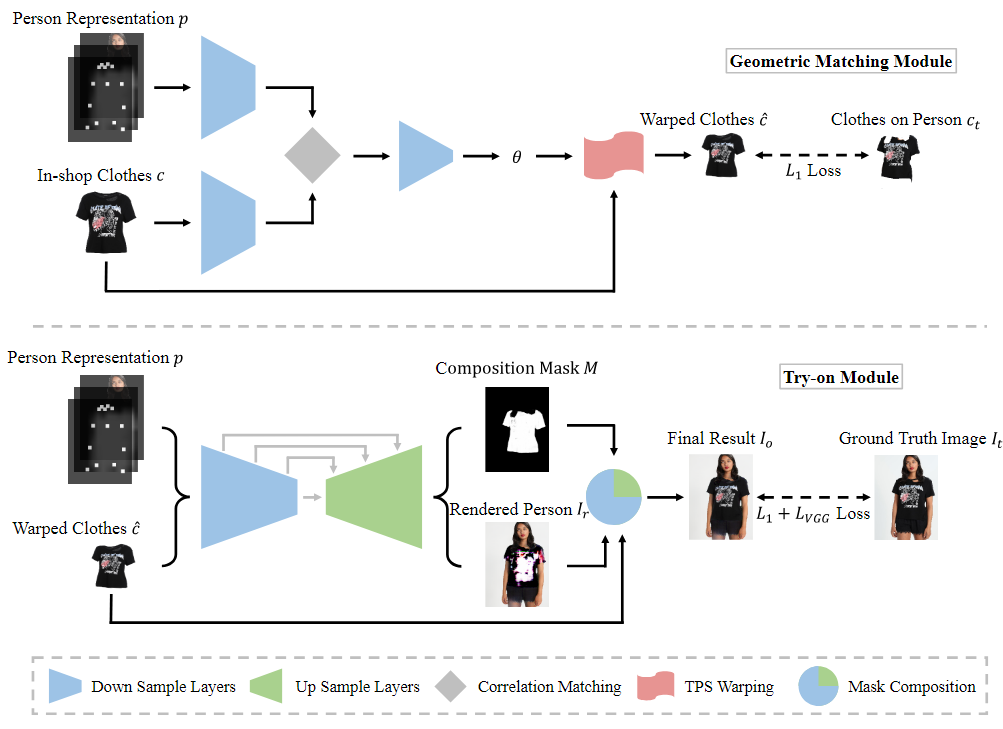
\includegraphics[width=0.85\linewidth]{content/resources/images/literature-review/cp-vton.png}
    \caption{Overview architecture of CP-VTON~\cite{Wang-ECCV2018-Toward}.}
    \label{vton-cpvton}
\end{figure}

Nonetheless, VITON~\cite{Han-CVPR2018-Viton} and CP-VTON~\cite{Wang-ECCV2018-Toward} only focus on deforming the target garment during the virtual try-on process. Consequently, these approaches lead to losing important details related to the human body when try-on. To mitigate this issue, Yang et al.~\cite{Yang-CVPR2020-Towards} proposed ACGPN, a framework that involves transforming the body-parser map to align with the target garment. Subsequently, the transformed parser map, input person image, and the deformed garment are utilized in the try-on generation. This integrated strategy ensures that the resulting try-on outcome effectively preserves the characteristics of both the human body and the in-shop clothes, enhancing the realism and fidelity of the try-on result.

\begin{figure}[h!]
    \centering
    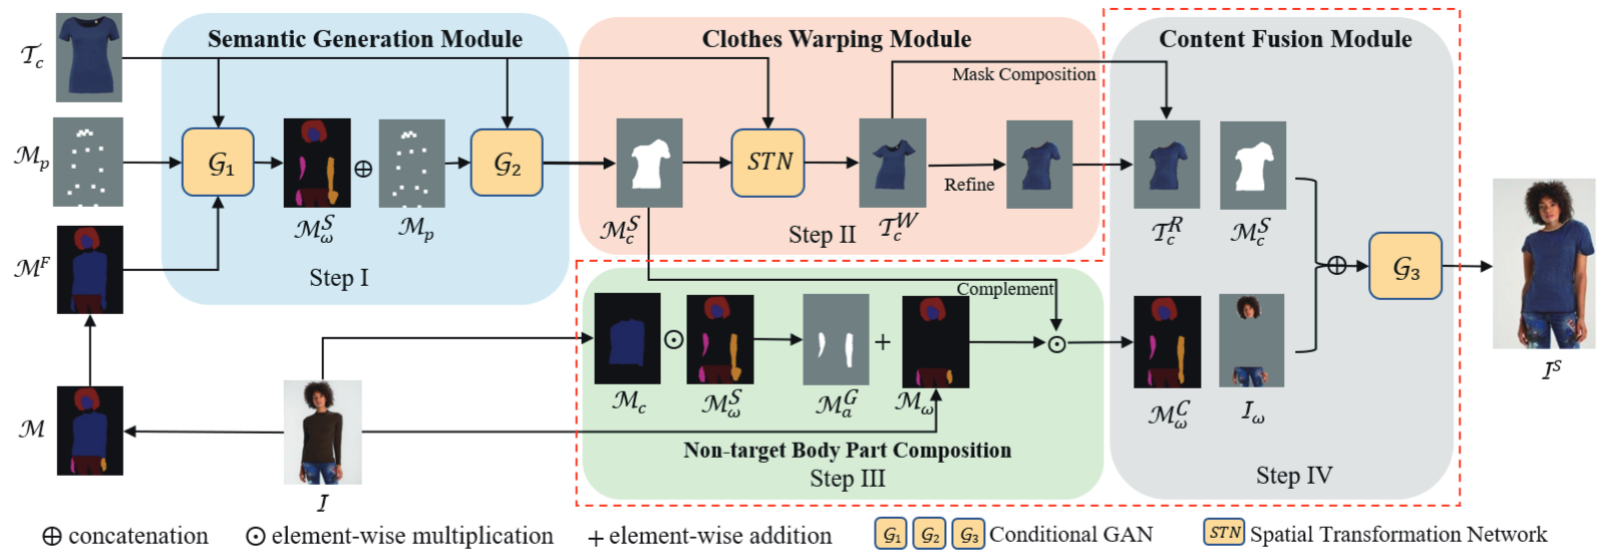
\includegraphics[width=\linewidth]{content/resources/images/literature-review/acgpn.png}
    \caption{Overview architecture of ACGPN~\cite{Yang-CVPR2020-Towards}.}
    \label{fig:vton-acgpn}
\end{figure}

Han et al.~\cite{Han-ICCV2019-Clothflow} introduced ClothFlow, a framework designed for synthesizing clothed person images, serving both posed-guided person image generation and virtual try-on tasks. First, similar to ACGPN~\cite{Yang-CVPR2020-Towards}, ClothFlow generates a segmentation map of the target person. Subsequently, a flow estimation network predicts the appearance flow~\cite{Zhou-ECCV2016-AppearanceFlow} that facilitates the warping of the source image to the desired target view. This approach yields more natural results compared to traditional TPS transformation. Finally, the final synthesized output is obtained by combining the source image, warped image, target segmentation map, and target pose. The ClothFlow framework for pose-guided person image generation is illustrated in~\autoref{fig:vton-clothflow}. For the virtual try-on tasks, the authors treated the garment image as the source image, and the input person pose as the target pose. The garment is then deformed by leveraging the predicted flow between the garment and the corresponding region of the person. The idea of using appearance flow instead of TPS transformation for deformation has been further developed and adopted by recent state-of-the-art methods~\cite{Ge-CVPR2021-Parser, He-CVPR2022-Style}.

\begin{figure}[h!]
    \centering
    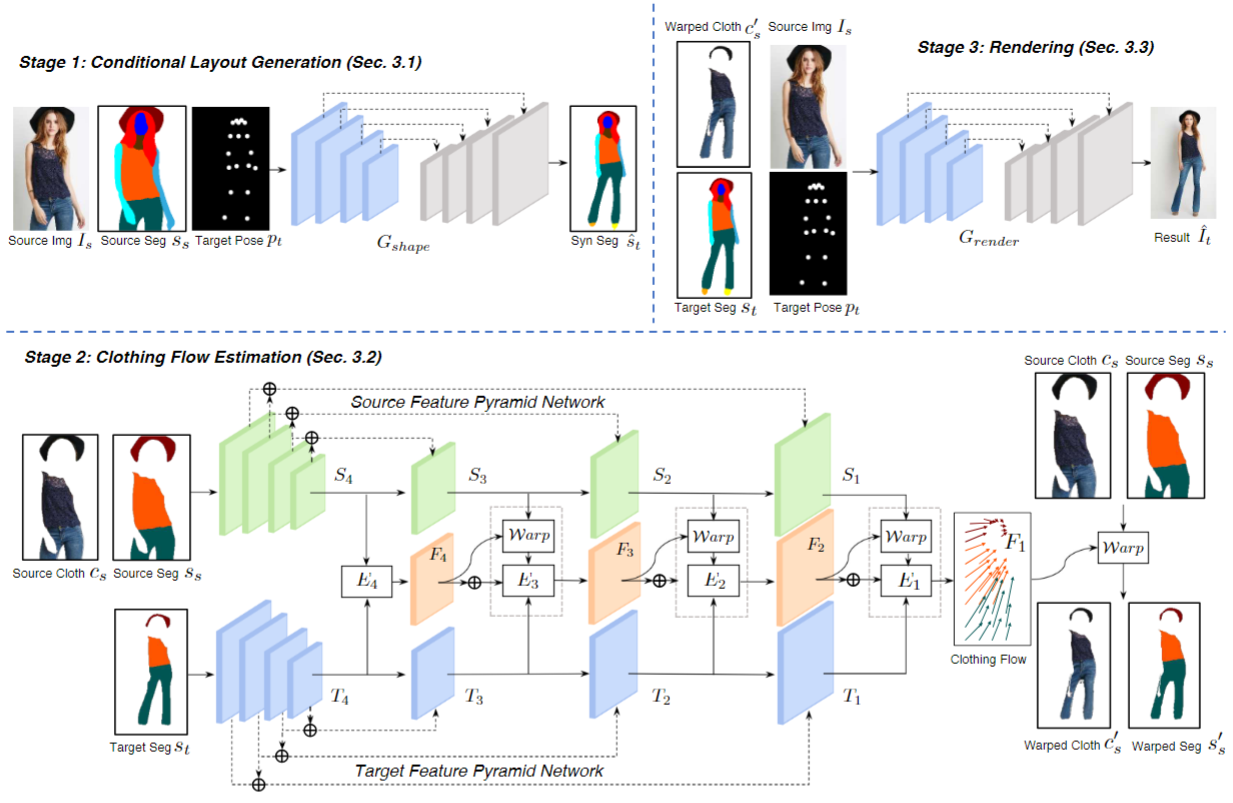
\includegraphics[width=\linewidth]{content/resources/images/literature-review/clothflow.png}
    \caption{Overview architecture of CLothFlow for pose-guided person image generation~\cite{Han-ICCV2019-Clothflow}.}
    \label{fig:vton-clothflow}
\end{figure}

Following the direction of multi-stage approaches, Fele et al.~\cite{Fele-WACV2022-CVTON} introduced a Context-driven Virtual Try-on Network (C-VTON). This framework comprises two fundamental components: a Body-Part Geometric Matcher, designed to deform the garment, and a Context-Aware Generator, aiming at generating the try-on image with contextual information.

\begin{figure}[h!]
    \centering
    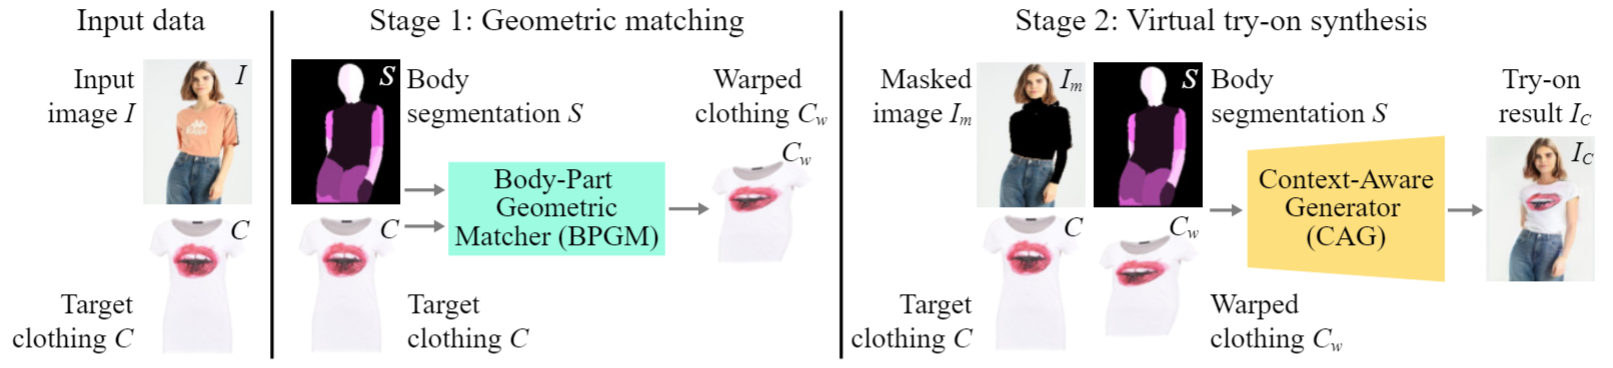
\includegraphics[width=\linewidth]{content/resources/images/literature-review/cvton.png}
    \caption{Overview architecture of C-VTON~\cite{Fele-WACV2022-CVTON}.}
    \label{fig:vton-cvton}
\end{figure}

However, the multi-stage approaches generate a try-on image relying on intermediate prediction results, which may be inaccurate, ultimately giving rise to noticeable artifacts in the final output. To address this issue, Bai et al.~\cite{Bai-ECCV2022-Single} introduced a novel Single Stage Virtual Try-on framework (SDAFN), which only uses a target pose map as guidance. By developing the deformable attention flow network and the shallow encoder and decoder, SDAFN allows the generation of try-on images end-to-end. The overall framework is shown in~\autoref{fig:vton-sdafn}.

\begin{figure}[h!]
    \centering
    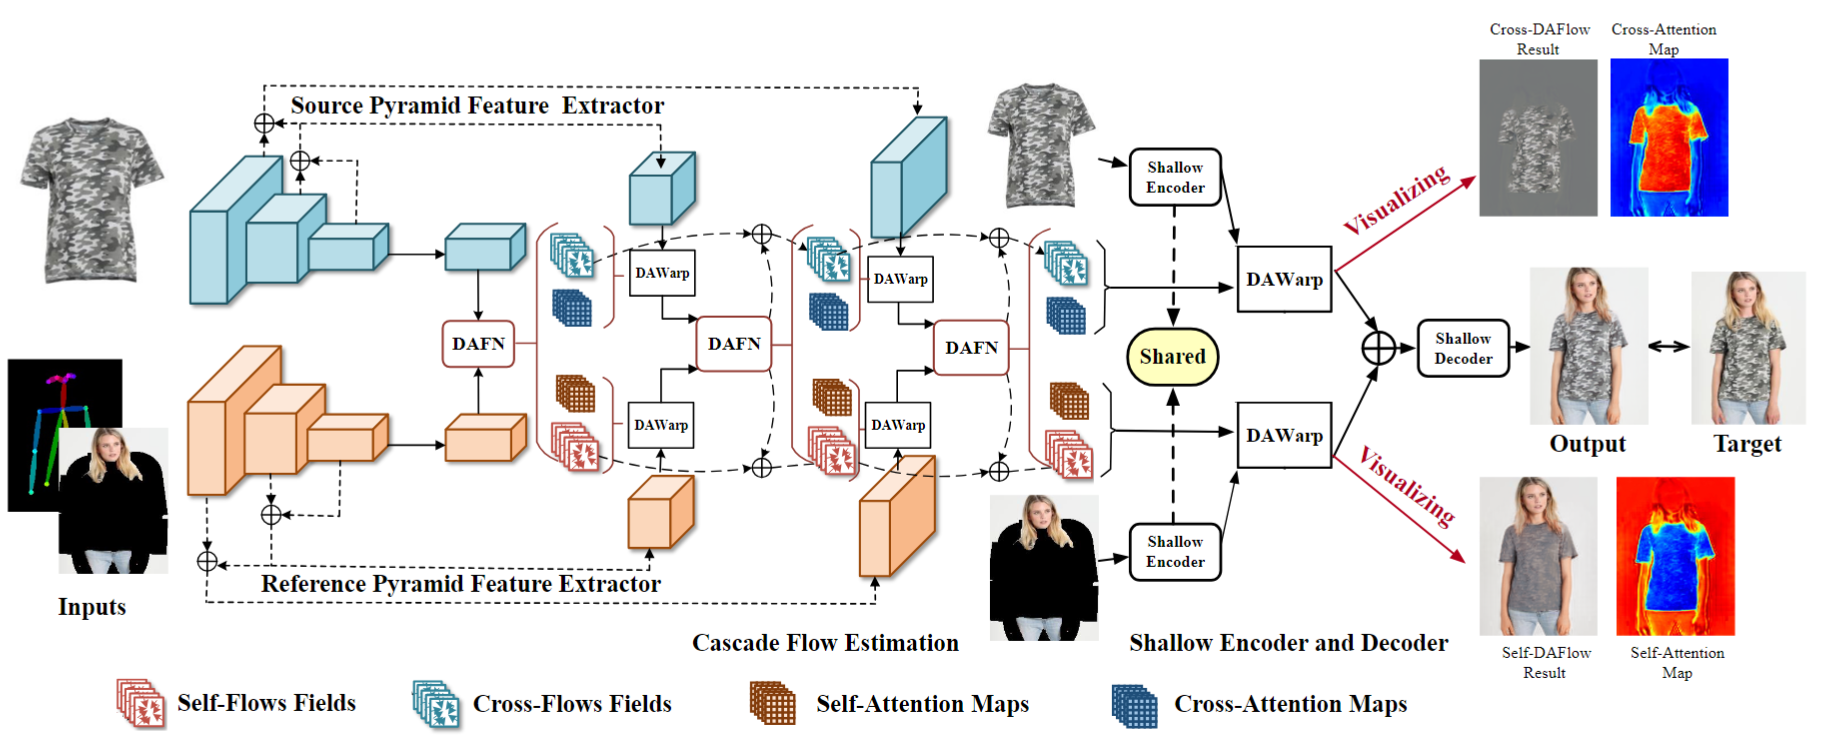
\includegraphics[width=\linewidth]{content/resources/images/literature-review/sdafn.png}
    \caption{Overview architecture of SDAFN~\cite{Bai-ECCV2022-Single}.}
    \label{fig:vton-sdafn}
\end{figure}

% \subsection{Parser-Free Approach}
\paragraph{Parser-free Methods.} In contrast, the parser-free approach only requires a person image and an input garment for inference. Consequently, this speeds up the process and eliminates reliance on human representation estimation models during inference. WUTON~\cite{Issenhuth-ECCV2020-Do}, as the pioneering parser-free method, introduced a Teacher-Student framework. It leverages a pretrained parser-based Teacher network to synthesize fake images acting as ground truth for guiding the training of the parser-free Student network.

\begin{figure}[h!]
    \centering
    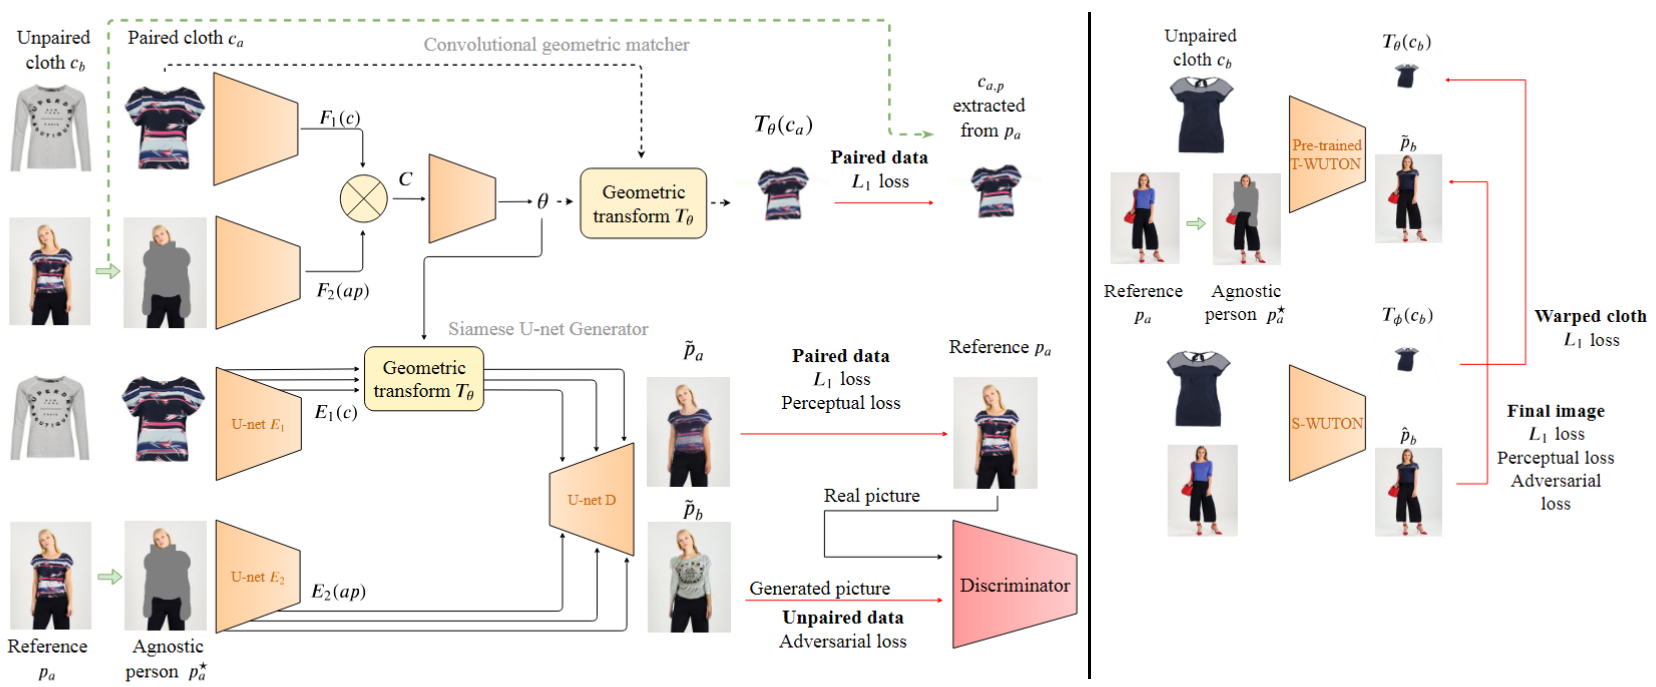
\includegraphics[width=\linewidth]{content/resources/images/literature-review/wuton.png}
    \caption{Overview architecture of WUTON~\cite{Issenhuth-ECCV2020-Do}.}
    \label{fig:vton-wuton}
\end{figure}

WUTON~\cite{Issenhuth-ECCV2020-Do} faces a specific limitation in which the optimization of the Student network is aimed at reconstructing synthetic images produced by the Teacher network. However, the result of the Teacher network has noticeable artifacts, resulting in a decline in the quality of the Student network. Ge et al.~\cite{Ge-CVPR2021-Parser} presented a novel knowledge distillation-based approach (PF-AFN) to overcome this challenge.  In this approach, the parser-free Student network uses the synthetic images generated by a parser-based network as input and learns to reconstruct the original images. By doing so, the training process of the Student network is supervised by real image data. This novel training method has since become the standard for subsequent parser-free methods.

\begin{figure}[h!]
    \centering
    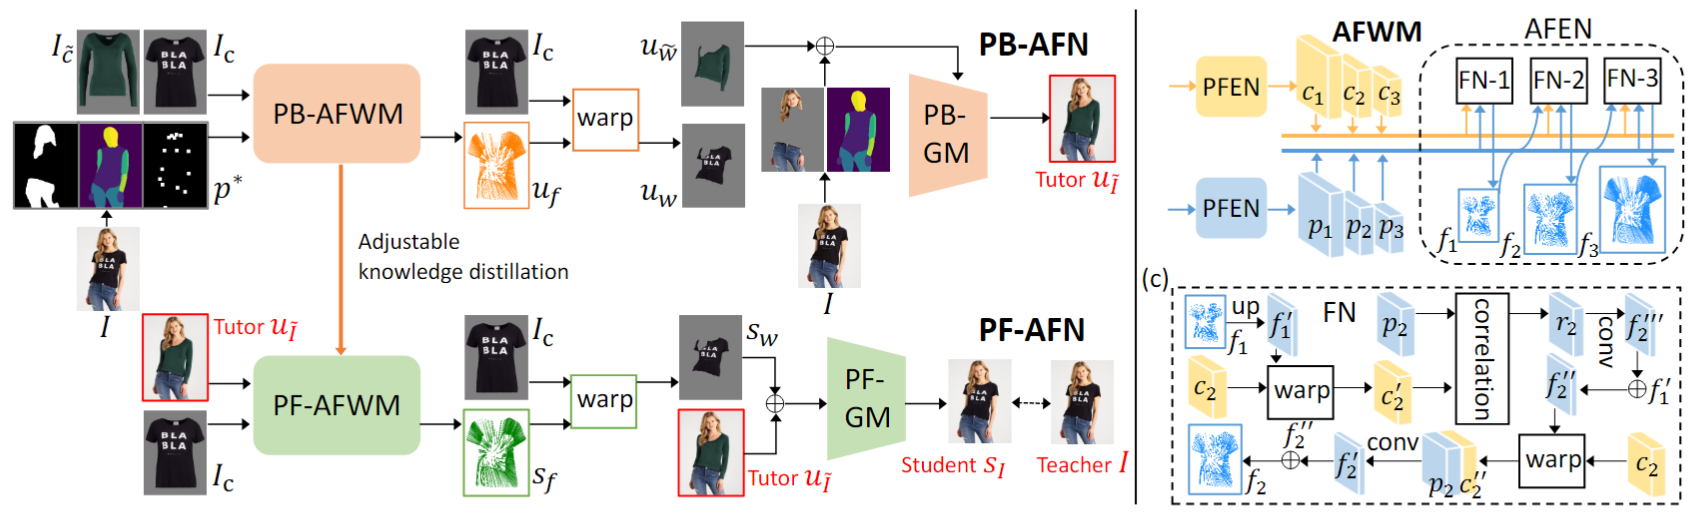
\includegraphics[width=\linewidth]{content/resources/images/literature-review/pfafn.png}
    \caption{Overview architecture of PF-AFN~\cite{Ge-CVPR2021-Parser}.}
    \label{fig:vton-pfafn}
\end{figure}

He et al.~\cite{He-CVPR2022-Style} proposed FS-VTON, an enhanced framework derived from PF-AFN~\cite{Ge-CVPR2021-Parser} with specific improvements in the warping component. The authors introduced a Style-based Global Appearance Flow Estimation using StyleGan blocks~\cite{Karras-CVPR2019-Style}. It enables the model to capture global and local correspondences between clothes and person images, enhancing garment deformation. In contrast, RMGN~\cite{Lin-IJCAI2022-RMGN} directed its focus towards the generation module through the development of a Regional Mask-Guided Generator, built upon SPADE blocks~\cite{Park-CVPR2019-Semantic} and residual connection.

\begin{figure}[h!]
    \centering
    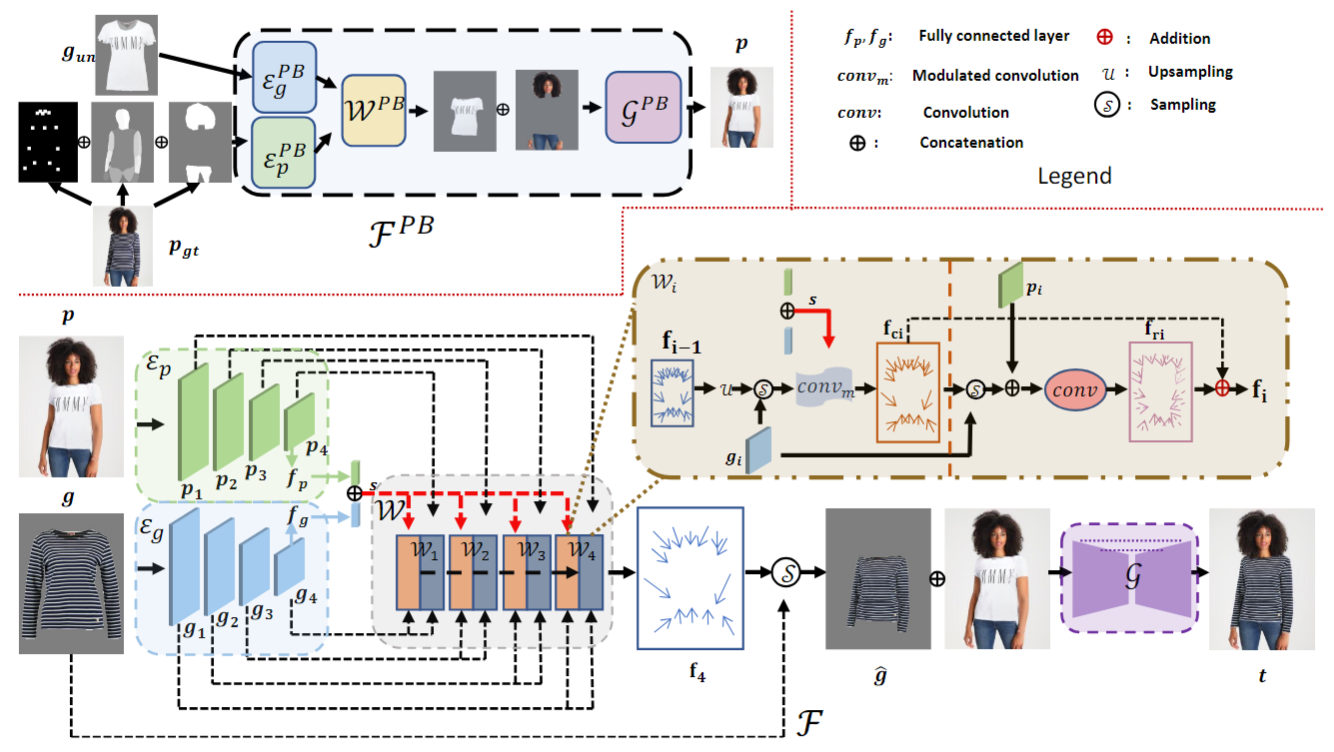
\includegraphics[width=\linewidth]{content/resources/images/literature-review/fsvton.png}
    \caption{Overview architecture of FS-VTON~\cite{He-CVPR2022-Style}.}
    \label{fig:vton-fsvton}
\end{figure}

\begin{figure}[h!]
    \centering
    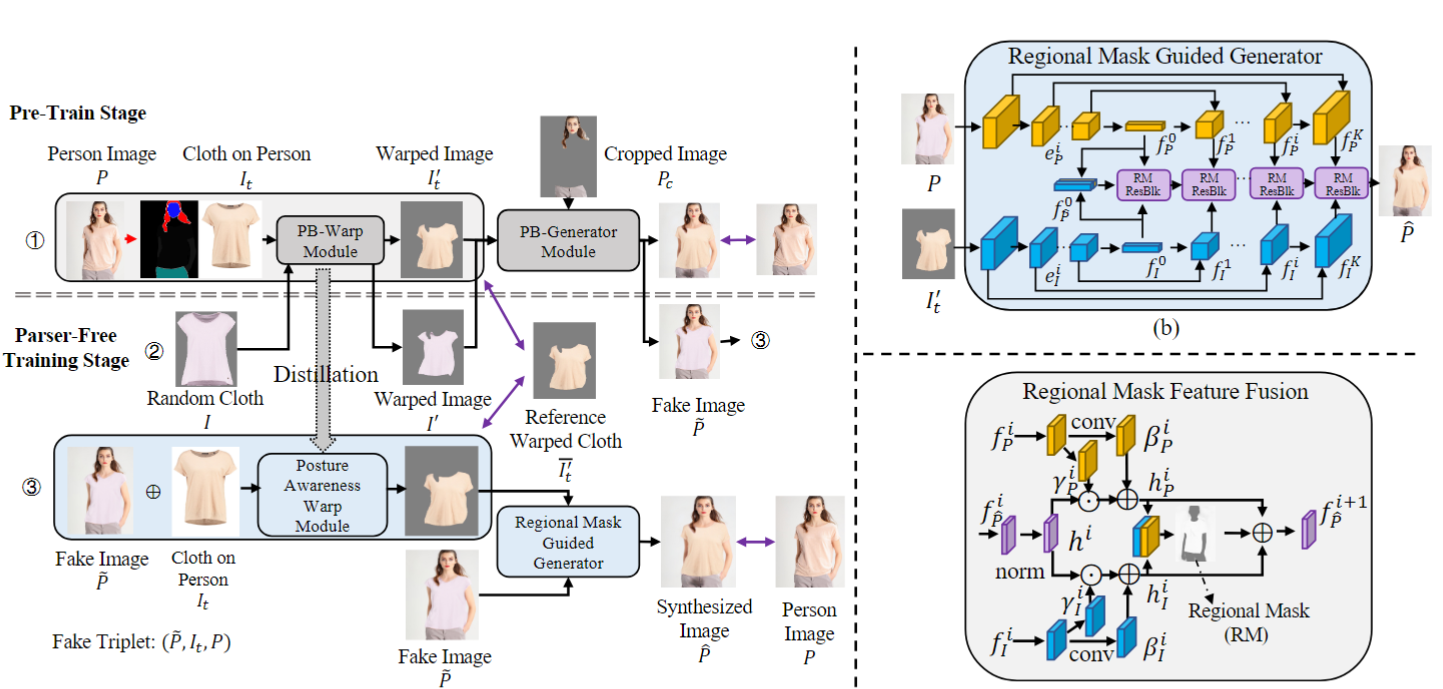
\includegraphics[width=\linewidth]{content/resources/images/literature-review/rmgn.png}
    \caption{Overview architecture of RMGN~\cite{Lin-IJCAI2022-RMGN}.}
    \label{fig:vton-rmgn}
\end{figure}


% \subsection{Video Virtual Try-on}
% \paragraph{Video Virtual Try-on.} There are also methods that aim to perform virtual try-on on a sequence of frames. These methods use techniques like memory-based~\cite{Zhong-ACMMM2021-Mvton} or optical flow~\cite{Kuppa-WACV2021-ShineOn} to keep the temporary consistency between the frames. However, these methods are still based on the parser-based approach, which takes considerable time to calculate the human representation. 

In this thesis, we adopt the parser-free approach to prioritize speed, as calculating human representation is a time bottleneck in the try-on process. However, we take a distinct step from existing methods by modifying the Student network for improved speed and reduced memory consumption while keeping the parser-based approach in the Teacher network to preserve the output quality.

\subsection{Commercial Products}
Companies are experiencing significant advancements in virtual try-on, offering many competitive advantages. Artificial intelligence (AI) and/or augmented reality (AR) are the technologies behind this technology. Such products are not limited to online platforms; even offline store owners can set up on-site kiosks or virtual mirrors,  enabling customers to try on items without risking damage to the actual product. In this part, we explore several commercial products already used by companies.

One example of a virtual try-on product is the virtual try-on for fashion accessories, exemplified by Warby Parker's pioneering initiative to provide customers with a virtual eyewear try-on experience~\cite{WarbyParker-Glasses}. Offering this feature on their website allows customers to experiment with different glasses styles before purchasing. This demand becomes even more important for high-end and costly products. Recognizing this, Baume \& Mercier, a luxury watch company, has enhanced their digital sales experience by incorporating a virtual try-on system~\cite{BaumeMercierr-TimeTide-Watch}.  Their method involves creating 3D watch models in various wrist sizes and striving to replicate transparency and lighting effects accurately~\cite{BaumeMercierr-Hapticmedia-Watch}.

\begin{figure}[h!]
    \centering
    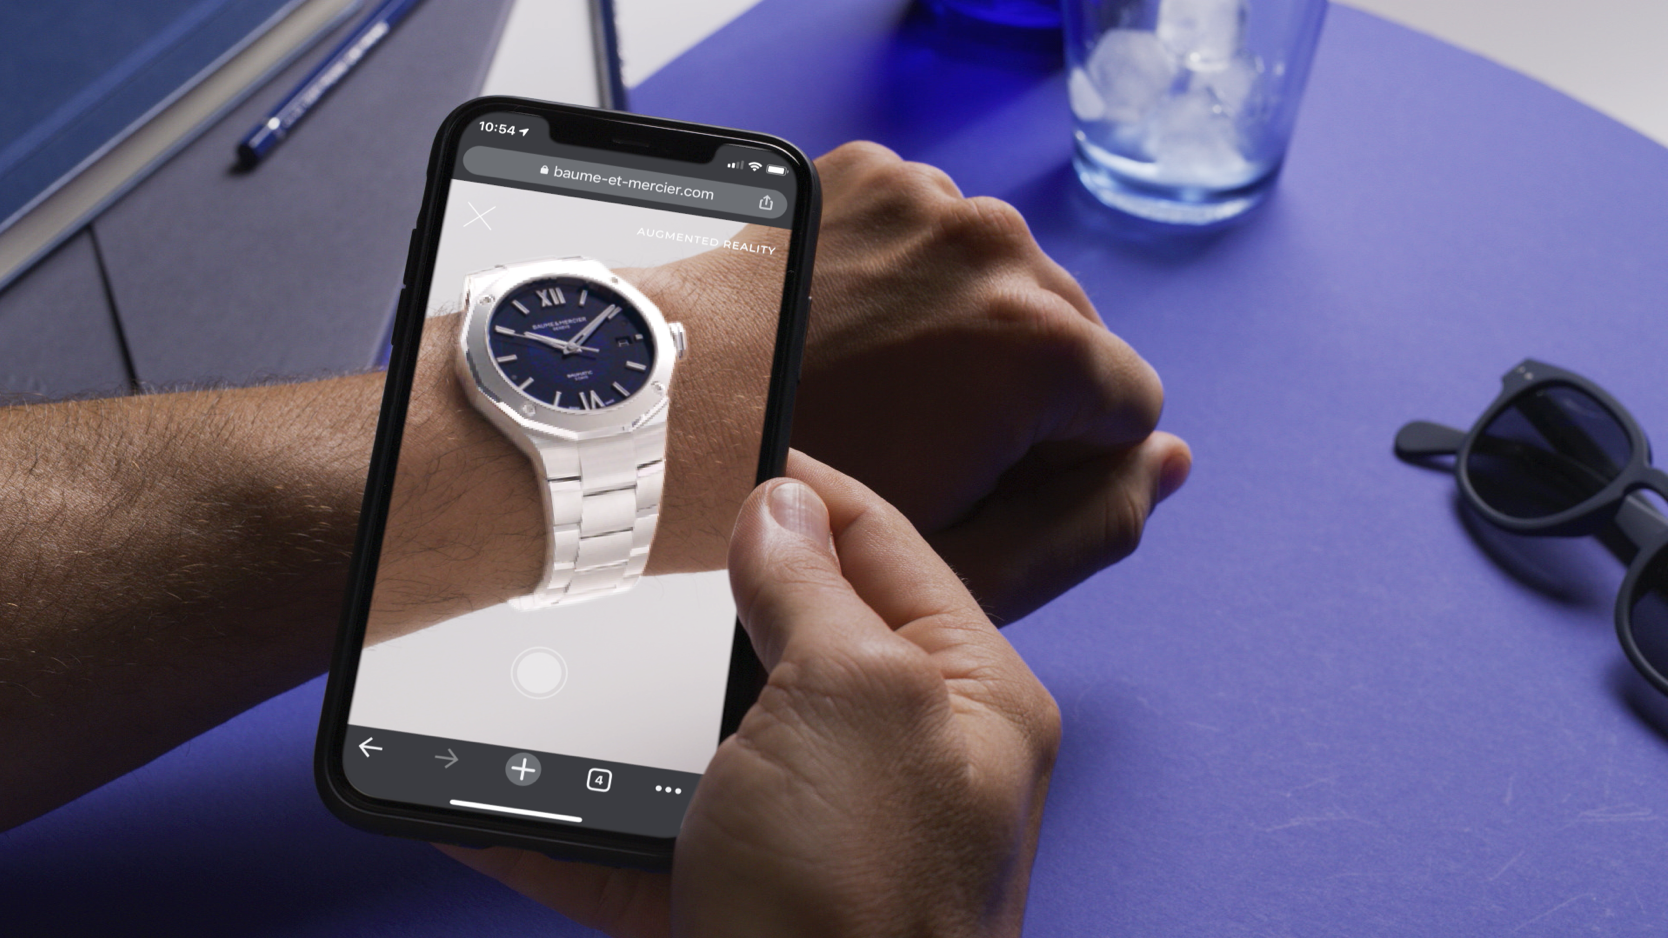
\includegraphics[width=\linewidth]{content/resources/images/literature-review/baume-mercier.png}
    \caption{Virtual try-on with 3D watch models (Source: Baume \& Mercier Virtual Try-On System ~\cite{BaumeMercierr-TimeTide-Watch}).}
    \label{fig:commercial-baume}
\end{figure}

Another awesome application is the virtual try-on for shoes, which leverages AR technologies to visualize how shoes appear on the user's feet. Some of the products that can be mentioned are Amazon virtual try-on for shoes~\cite{AmazonVTO-Aboutamazon2022-Shoes} and Artlabs~\cite{Artlabs-Shoes}, which can fit 3D shoe models onto the customer's feet. Consequently, customers can assess the appearance of the shoes from multiple angles by moving their feet.

The virtual try-on for clothes is another challenge. The methods employed in this domain aim to fit the clothes to suit the target human pose. Compared to the 3D-based solutions, which wear the 3D model of the item to the customer's body~\cite{GeeneeVTO-Clothes} or allow users to create 3D models that represent them to try on~\cite{ZalandoVTO-Zalando2023-Clothes}, the 2d-based virtual try-on product (e.g. Google Shopping virtual try-on~\cite{GoogleVTO-GoogleBlog2023-Clothes}), which use the real models and direct processing on the image, is intensively developing and applying over the years. However, Google Shopping's virtual try-on feature~\cite{GoogleVTO-GoogleBlog2023-Clothes} only allows users to select from the available model images, which makes it difficult for customers who wish to evaluate the fit of items on their bodies.

\begin{figure}[h!]
    \centering
    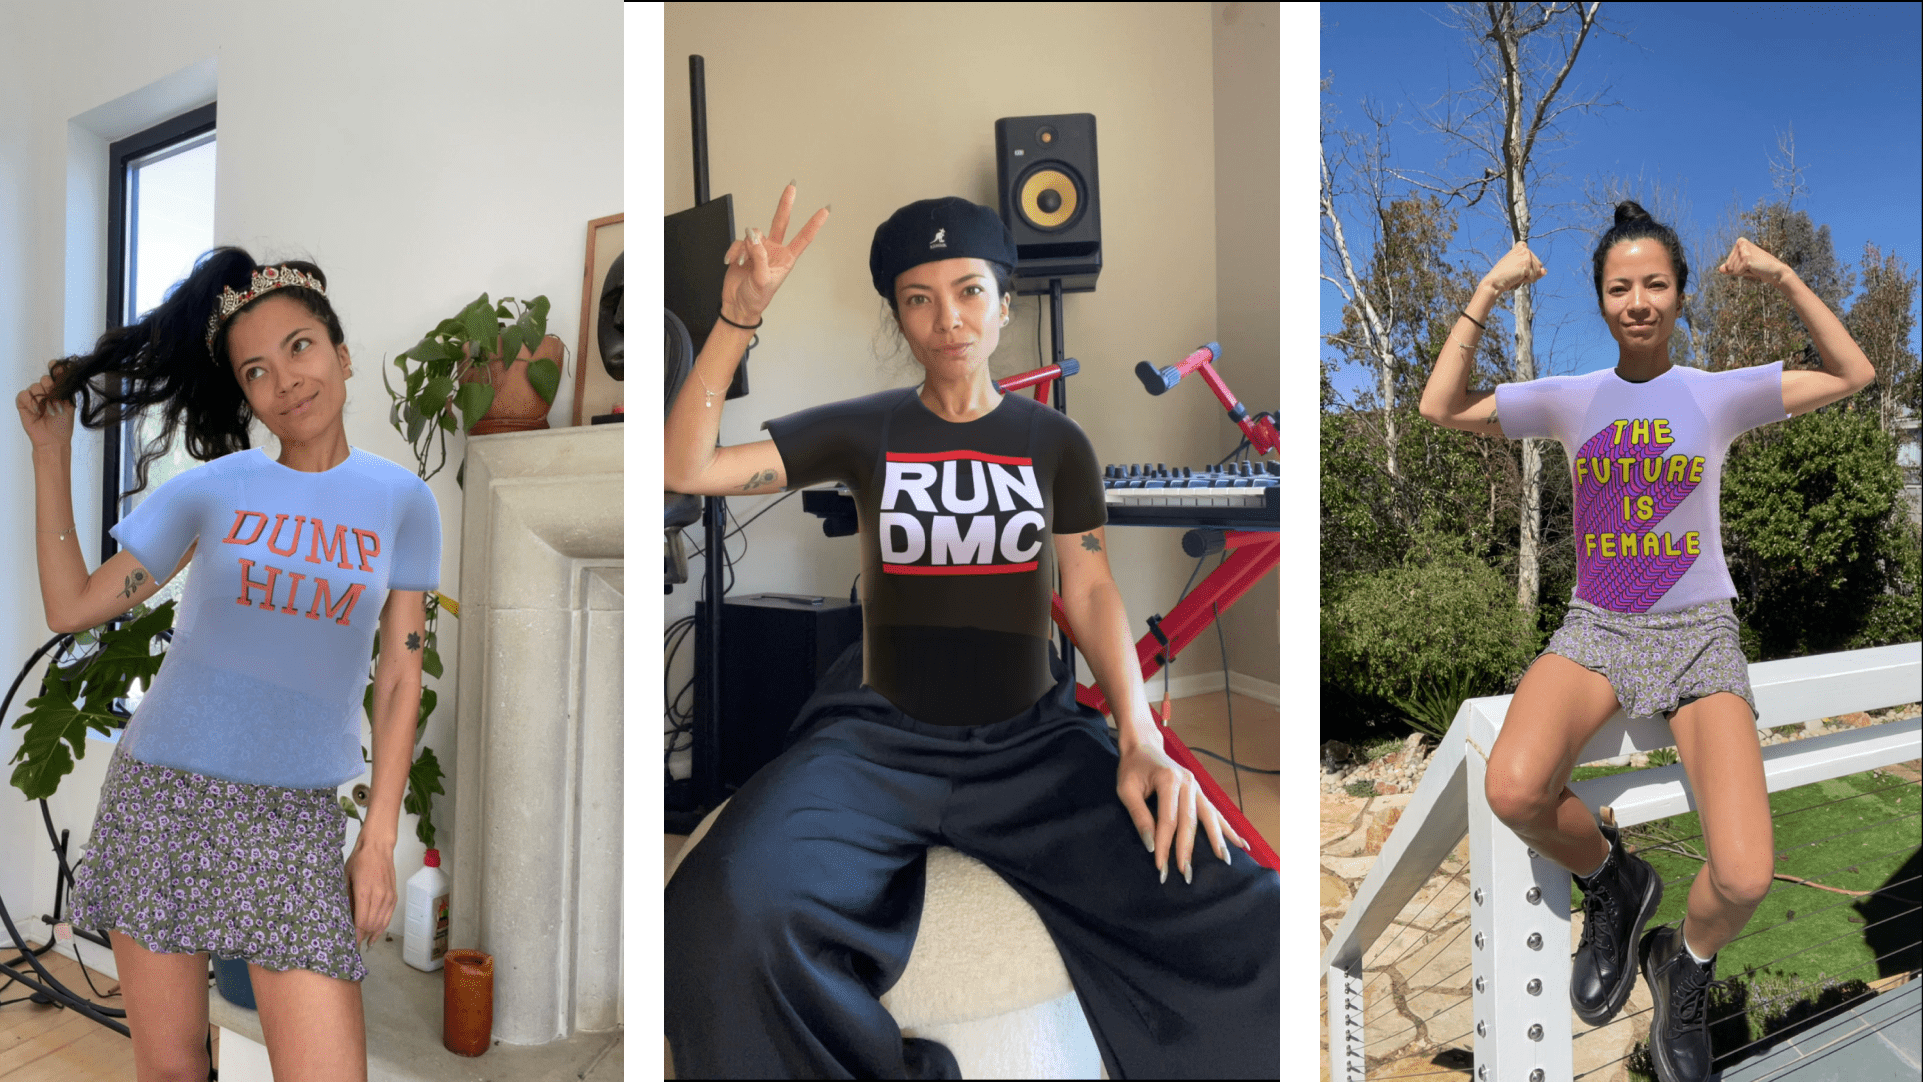
\includegraphics[width=\linewidth]{content/resources/images/literature-review/geenee-ar.png}
    \caption{Tracking human body to wear 3D clothes models (Source: Geenee AR~\cite{GeeneeVTO-Clothes}).}
    \label{fig:commercial-amazon}
\end{figure}

\begin{figure}[h!]
    \centering
    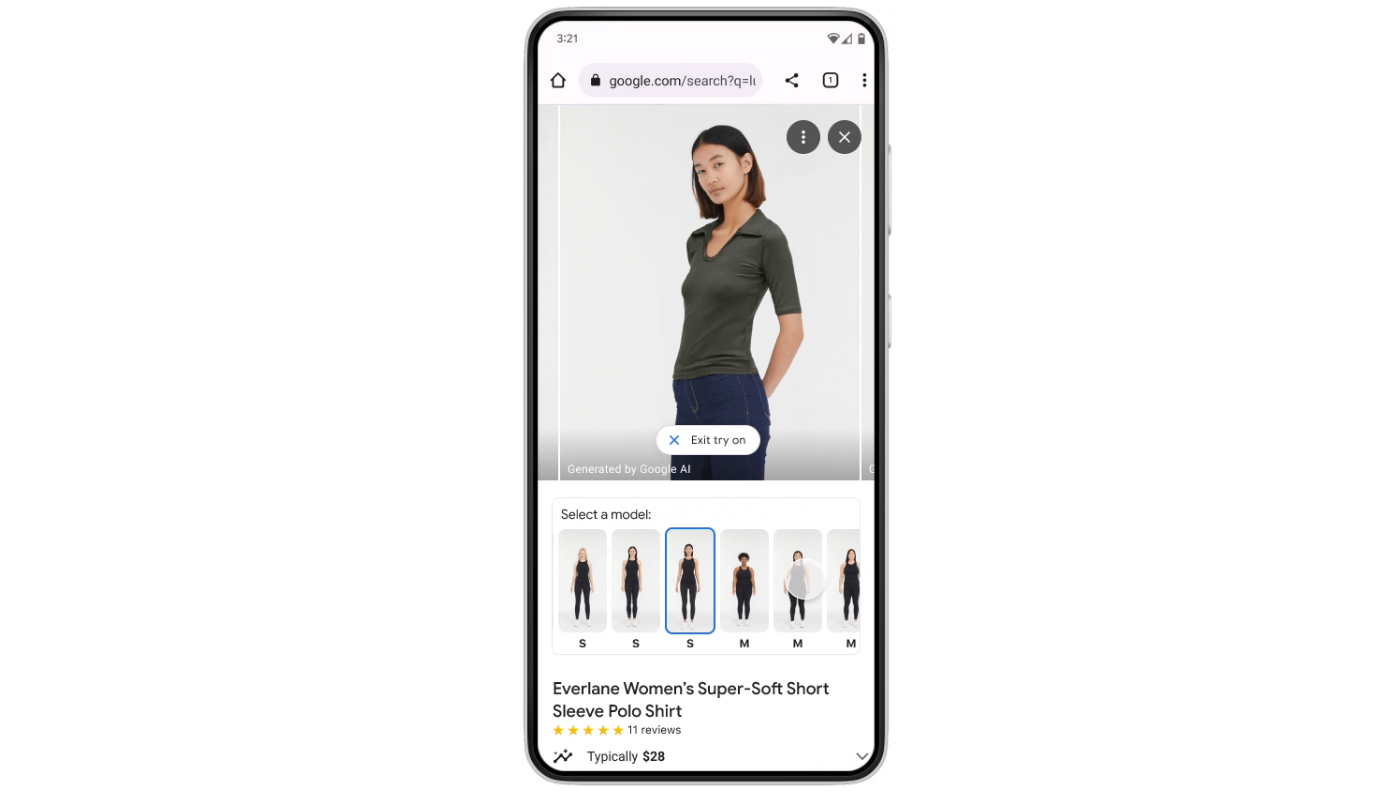
\includegraphics[width=\linewidth]{content/resources/images/literature-review/google-tryon.png}
    \caption{Google AI virtual try-on feature for shopping (Source: Google introduces new AI virtual try-on feature~\cite{GoogleVTO-GoogleBlog2023-Clothes}).}
    \label{fig:commercial-google}
\end{figure}

% Within the scope of this thesis, we focus on how virtually try-on clothes, specifically upper-body clothes. 

 %%%%%%%%%%%%%%%%%%%%%%%%%%%%%%%%%%%%%%%%%%%%%%%%%%%%%%%%%%%%%%%%
 \newpage
\section{Fashion Recommendation}
With the explosion of data and deep learning, a growing number of studies have focused on visual-based fashion recommendations. 
In 2018, Mariya et al.~\cite{Mariya-ECCV18-Learning} provided the PolyvoreOutfits dataset to support the fill-in-the-blank task, where we need to find an item of a specific category to complete a partial outfit. 
\begin{figure}[h!]
    \centering
    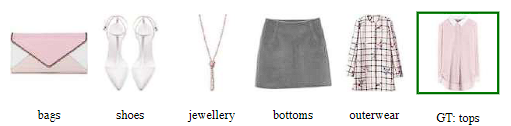
\includegraphics[width=0.6\linewidth]{content/resources/images/literature-review/fitb.PNG}
    \caption{Outfit fill-in-the-blank task, where the highlighted item is the missing item (Source: Fashion Outfit Complementary Item Retrieval~\cite{Lin-CVPR2020-Fashion}).}
    \label{fig:fitb-task}
\end{figure}

They also propose a Type-Aware network (\autoref{fig:type-aware}) as the baseline framework. 
Initially, the framework learns a shared embedding space where all fashion items are represented. Subsequently, this shared embedding space is projected into subspaces based on pairs of item types. For example, in the top-shoes subspace, the shoes that match a specific top must be close, even if they differ significantly in the overall embedding space.

\begin{figure}[h!]
    \centering
    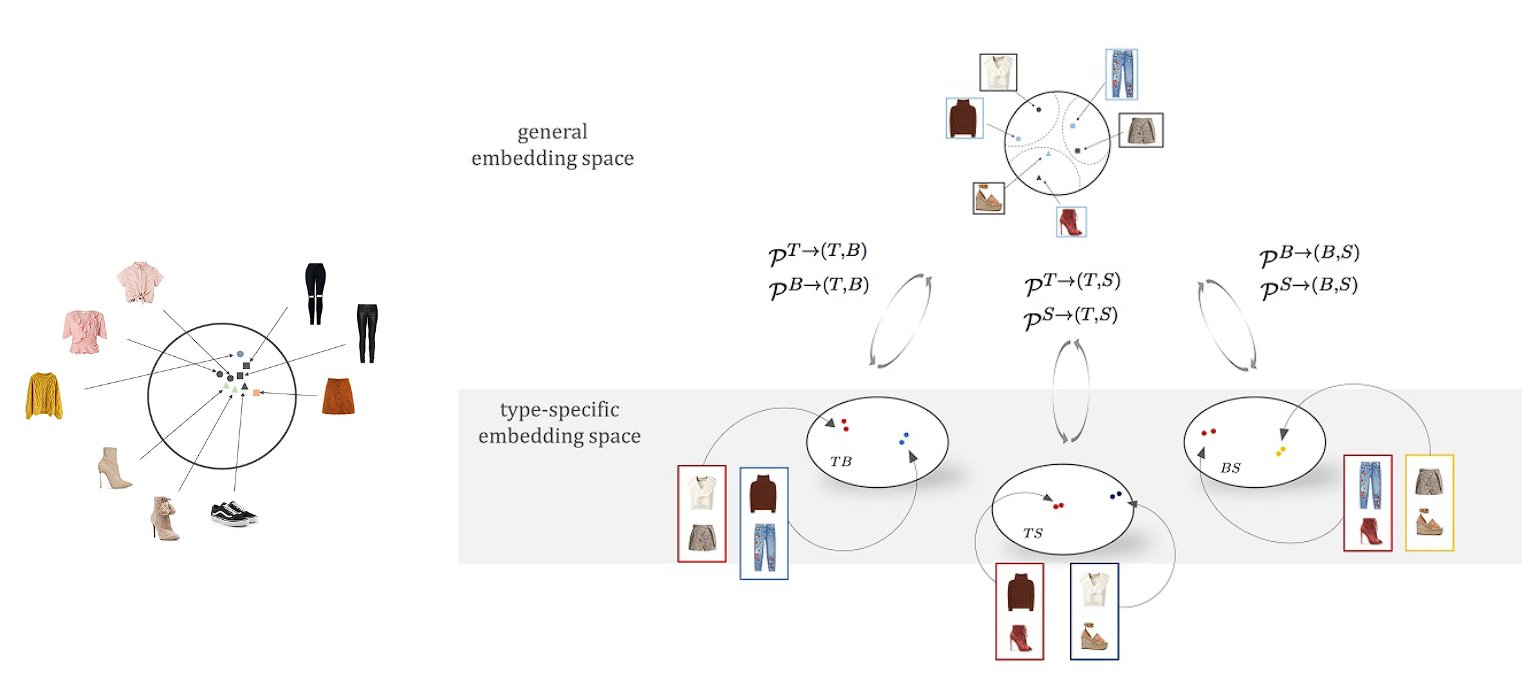
\includegraphics[width=\linewidth]{content/resources/images/literature-review/TypeAware.PNG}
    \caption{Type-Aware learning strategies (Source: Learning Type-Aware Embeddings for Fashion
Compatibility~\cite{Mariya-ECCV18-Learning}).}
    \label{fig:type-aware}
\end{figure}

After the Self-Attention mechanism and Transformers architecture \cite{Vaswani-NeurIPS2017-Attention} were introduced and gained success in the natural language processing task~\cite{Devlin-ArXiv2018-BERT}, CSA-Net~\cite{Lin-CVPR2020-Fashion} and OutfitTransformer~\cite{Sarkar-CVPRW2022-OutfitTransformer} incorporated these ideas by utilizing the textual embeddings of the categories and significantly improved the recommendation results. 

\begin{figure}[h!]
    \centering
    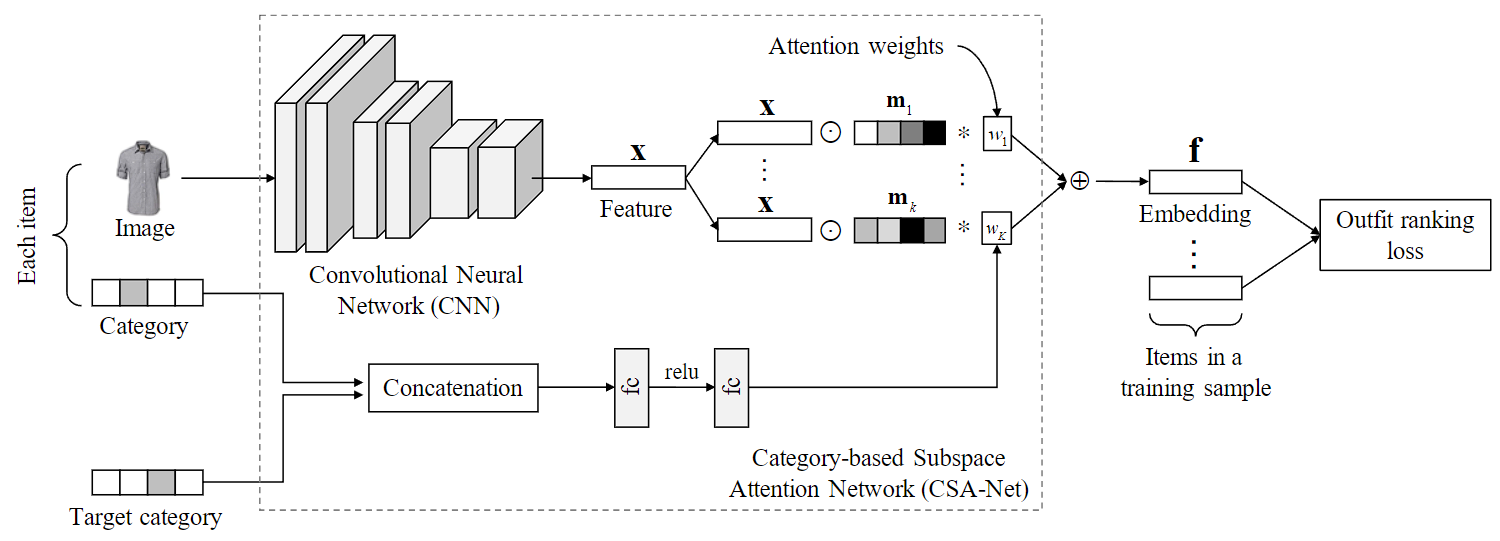
\includegraphics[width=\linewidth]{content/resources/images/literature-review/CSA.PNG}
    \caption{Overview of CSA-Net framework (Source: Fashion Outfit Complementary Item Retrieval~\cite{Lin-CVPR2020-Fashion}).}
    \label{fig:csa}
\end{figure}

Specifically, CSA-Net represents each category by an embedding vector to capture their textual semantics. The CSA-Net framework (illustrated in \autoref{fig:csa}) takes a reference image, its category vector, and a target category vector. A Convolution Neural Network is employed to extract the image embedding. This vector is then multiplied by a set of masks to create multiple subspace embeddings (multi-attention head). The concatenated category vector is used to predict the attention weights, which determine the contribution of each subspace embeddings in the final output embedding.

To eliminate the learning of pair-wise embeddings in the above methods, OutfitTransformer~\cite{Sarkar-CVPRW2022-OutfitTransformer} learns the embedding of an entire outfit by utilizing the Transformer Encoder block and a special token at the first position (same as \textit{<CLS>} token in BERT~\cite{Devlin-ArXiv2018-BERT}). This token not only captures the embeddings of all items in the outfit but also specifies the target category for the missing item (as shown in \autoref{fig:outfittransformer}).

\begin{figure}[h!]
    \centering
    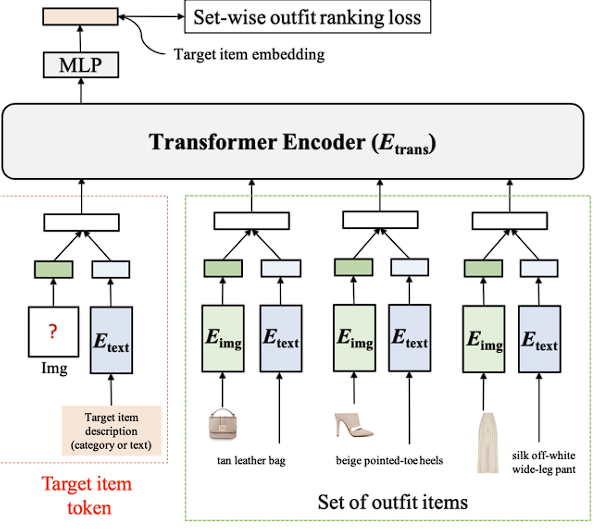
\includegraphics[width=0.6\linewidth]{content/resources/images/literature-review/OutfitTransformers.PNG}
    \caption{Overview of OutfitTransformer framework (Source: OutfitTransformer: Outfit Representations for Fashion Recommendation~\cite{Sarkar-CVPRW2022-OutfitTransformer}).}
    \label{fig:outfittransformer}
\end{figure}

Wu et al.~\cite{Wu-CVPR2021-FashionIQ} further expanded the research scope by introducing the FashionIQ dataset for the text feedback-guided item retrieval task, where we need to find the desired item given a reference input item and its relative attribute feedback in the natural language. \autoref{fig:fashioniq} demonstrates the retrieval pipeline based on the user's feedback.

\begin{figure}[h!]
    \centering
    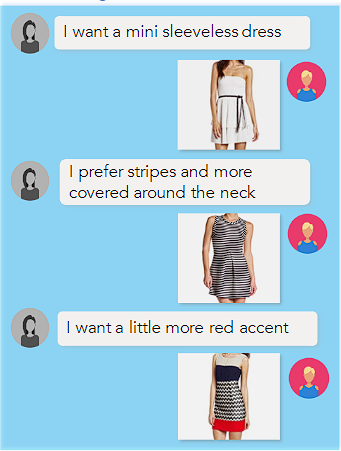
\includegraphics[width=0.4\linewidth]{content/resources/images/literature-review/fashioniq.PNG}
    \caption{Demonstration of feedback-guided retrieval (Source: Fashion IQ: A New Dataset Towards Retrieving Images by Natural Language Feedback~\cite{Wu-CVPR2021-FashionIQ}).}
    \label{fig:fashioniq}
\end{figure}

By utilizing CLIP~\cite{Radford-OpenAIblog2019-Language}, a deep learning model that learns the joint representations of both images and textual descriptions, Baldrati et al. \cite{Baldrati-CVPR2022-Effective, Baldrati-CVPR2022-Conditioned} achieved state-of-the-art performance on the FashionIQ dataset, proving its applicability to the fashion domain for text feedback-guided image retrieval. 

\begin{figure}[h!]
    \centering
    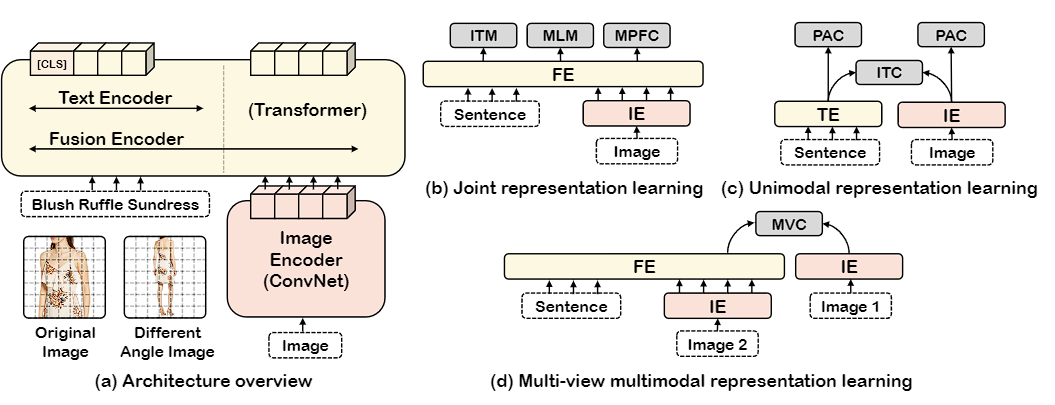
\includegraphics[width=\linewidth]{content/resources/images/literature-review/fashionvil.PNG}
    \caption{Overview of FashionViL architecture (Source: FashionViL: Fashion-Focused
Vision-and-Language Representation Learning~\cite{Han-ECCV2022-FashionViL}).}
    \label{fig:fashionvil}
\end{figure}

Han et al.~\cite{Han-ECCV2022-FashionViL} bridged the gap between the text feedback-guided image retrieval problem and the fill-in-the-blank problem by proposing a general vision-and-language network framework. The FashionViL overall architecture is shown in~\autoref{fig:fashionvil}. The framework optimizes its text and image encoders by learning multiple tasks such as Multi-view contrastive learning (MVC), Pseudo-attribute classification (PAC), Masked patch feature classification (MPFC), Image-text contrastive learning (ITC), Image-text matching (ITM), and Masked language modelling (MLM). Subsequently, the framework encoders can produce universal embeddings for downstream tasks such as text feedback-guided image retrieval or fill-in-the-blank problem.
 %%%%%%%%%%%%%%%%%%%%%%%%%%%%%%%%%%%%%%%%%%%%%%%%%%%%%%%%%%%%%%%%
\section{Similarity Search}
Similarity search has become a hot topic in recent years due to the explosion of data. There are two main types of similarity search: exhaustive and approximate. Exhaustive searching, such as the K-Nearest Neighbor (KNN) algorithm, involves calculating the distances between the query point and all items in a dataset to find the nearest neighbours. This approach provides accurate results but can be computationally expensive, especially in large datasets or high dimensional data points.

Approximate searching rises as the solution for the time complexity of exhaustive searching. These methods either reduce the dataset dimension or limit the search scope with the trade-off for accuracy. Production Quantization (PQ)~\cite{Jegou-TPAMI2010-Product} clusters each dimension or group of dimensions into buckets and indexes the dataset by those buckets instead, thus reducing the number of bytes required to represent the dataset (as illustrated in \autoref{fig:product-quantization}).

\begin{figure}[h!]
    \centering
    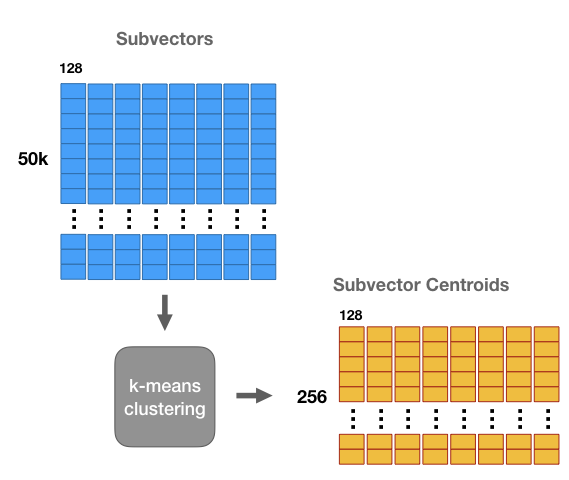
\includegraphics[width=0.6\linewidth]{content/resources/images/literature-review/kmeans_clustering.png}
    \caption{Overview of Production Quantization method (Source: Product Quantizers for k-NN Tutorial Part 1~\cite{web-pq}).}
    \label{fig:product-quantization}
\end{figure}

In terms of limiting the search scope, Inverted File Index (IVF)~\cite{Sivic-ICCV2003-Video} divides the search space into subspaces and only searches in a subset of these subspaces. Some methods leverage the tree~\cite{Erik-Github-Annoy} or graph~\cite{Malkov-TPAMI2018-Efficient} data structure to speed up the search process with the cost of more memory consumption. Specifically, Hierarchical Navigable Small Worlds~\cite{Malkov-TPAMI2018-Efficient} constructs multiple subgraphs from all items; the lower the level is, the denser the subgraph becomes, and the searching process is performed like in a Skip List. Approximate Nearest Neighbors Oh Yeah~\cite{Erik-Github-Annoy} builds a binary tree by repeatedly choosing two random items and splitting the space into two subspaces; Spotify's recommendation system uses this algorithm.